%
% tp1.tex
%
% auteurs: Paul Chabanon (PC) et Antoine Guerrée (AG)
% créé le: 2013-06-01
% dernière mise-à-jour: 2013-06-01
%
% Description:
% Fichier principal du document. Contient les commandes LaTeX nécessaires,
% et inclus les autres fichiers nécessaires au rapport.
% Pour compiler ce document, les packages texlive et texlive-lang-french
% texlive-latex-extra sont recommandés.
%


%% En-tête
\documentclass[a4paper,12pt,titlepage]{article}
\usepackage[french]{babel}
\usepackage[utf8]{inputenc} % encodage
\usepackage[T1]{fontenc} % encodage
\usepackage{array} % tableaux
\usepackage[bookmarks=true,colorlinks,linkcolor=blue]{hyperref} % hyperliens
\usepackage{aeguill} % lisibilité
\usepackage{graphicx} % pour insérer des images
\usepackage{amssymb,amsmath} % maths
\usepackage{multicol} % colonnes
\usepackage[francais]{varioref} % chouettes refs
\usepackage{listingsutf8} % to allow utf8 with lstlisting
\usepackage{amsthm} % math proof
\usepackage{float} % mettre les figures où on veut

\lstset{ 
  language=C++,        
  tabsize=3,              
  showstringspaces=false, %pour virer les espaces dans les chaines de caractères
  %basicstyle=\ttfamily\footnotesize,
  %commentstyle=\color{Green}\scriptsize, % white comments
  %keywordstyle=\bfseries,
	%keywordstyle=\color{Blue}\textnormal,
	keywordstyle=\bfseries\ttfamily\color[rgb]{0,0,1},
	identifierstyle=\ttfamily,
	commentstyle=\color[rgb]{0.133,0.545,0.133},
	stringstyle=\ttfamily\color[rgb]{0.627,0.126,0.941},
	showstringspaces=false,
	basicstyle=\small,
	numberstyle=\footnotesize,
  title=\lstname, %afficher le titre
  frame=leftline, % le cadre
  captionpos=b, %légende en dessous
  numbers=left, %pour rajouter des numéros de ligne
  stepnumber=5, %définition du pas pour les numéros
  firstnumber=1, %définition du 1er numéro
  breaklines=true,      %pour casser les lignes trop longues
  caption=\lstname,
  inputencoding=utf8/latin1
}


%% Propriétés du document
\title{Compte-rendu de projet IF23\\Système autonome de manipulation de données GPS}
\author{Youenn Piolet \and Julien Nozais \and Alexandre Horréard}
\date{\today} % préférer la date réelle du TP


\begin{document}

\maketitle

\tableofcontents

\newpage

\section{Présentation du projet}

Le but du projet était de créer le programme tournant sur un micro-contrôleur Arduino permettant de manipuler des données GPS.

Notre boitier récupère les informations envoyées par le module GPS et les stockent sur une carte SD dans des fichiers. 
Ces fichiers peuvent ensuite être récuperés sur un PC pour être utilisés avec GPSprune, un logiciel permettant d'afficher
le parcours correspondant aux données envoyées.

\medskip
Un premier bouton permet de demarrer ou d'arreter le parcours. Chaque nouveau redemarage créé un nouveau fichier où enregistrer les données.
Chaque parcours est donc enregistré dans un fichier separé. On peut également mettre le parcours sur pause et le redemmarer ensuite, sans changer de parcours.

Le boitier dispose d'un écran LCD qui permet d'afficher plusieurs informations. En appuyant sur un deuxième bouton on change l'affichage.
L'écran peut afficher les coordonnées, la vitesse, la distance parcourue ou l'heure. Toutes ces informations sont bien evidement mises à jour en temps réel.

Un autre bouton permet de choisir le mode d'enregistrement : soit les points sont enregistrés suivant un temps fixe (toutes les trois secondes),
soit les points sont enregistrés suivant leur distance avec le point d'avant. Nous obtenons ainsi une suite de point qui ne sont pas identiques.

L'ensemble fonctionne sur pile. Au demarrage du boitier, la batterie s'affiche sur l'écran LCD.


\section{UML}

\subsection{Diagramme de cas d'utilisation}

\begin{figure}[H]
	\centering
	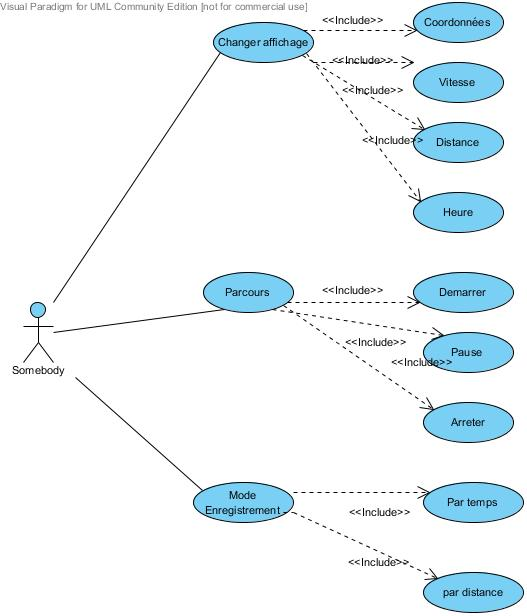
\includegraphics[width=\textwidth]{use_case.jpg}
	\caption{Diagramme de cas d'utilisations}
	\label{usecase}
\end{figure}

\subsection{Diagramme de séquence}

\begin{figure}[H]
	\centering
	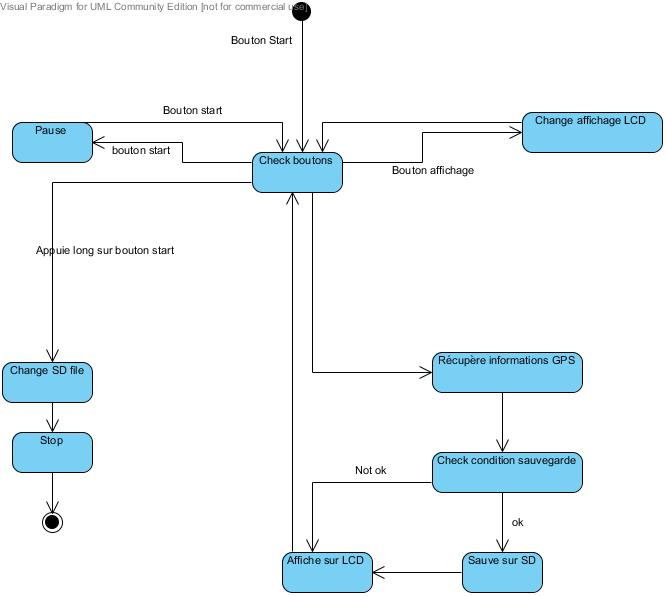
\includegraphics[width=\textwidth]{sequence.jpg}
	\caption{Diagramme de séquence}
	\label{sequence}
\end{figure}

\section{Fonctionnement du programme}

\subsection{Fonctionnement général}

L'affichage sur écran LCD, le système de navigation, la sauvegarde sur carte SD et la récupération des données du module GPS sont tous géré par des classes séparées.
La boucle principale ne fait qu'appeler les fonctions des instances de ces classes dans l'ordre. Cette boucle principale gère aussi le fonctionnement des boutons.
A chaque passage dans la boucle le système teste si un des boutons à été appuyé et suivant quel bouton a été appuyé il lance la methode indiqué.

\subsection{Gestion du GPS}

Le module GPS est géré par la classe GPShandler.
La fonction principale de cette classe est \emph{refreshData}.
Cette fonction récupère les informations du modules GPS grace à une liaison série et la fonction \emph{encode}.
Une boucle permet de récuperer tous les caractères qui arrivent de la liaison série.
La fontion \emph{encode} permet de tester si toute la trame est arrivé, en effet elle ne renvera vrai que si elle arrive à décoder la trame. Sinon la trame n'est pas complète on continue de tourner dans la boucle.

Lorsque toute la trame est arrivé, on met à jour ses attributs privés \emph{\_lat}, \emph{\_lon}, \emph{\_date}, \emph{\_time} et \emph{\_speed}.
Pour gérer les problèmes dans la transmission, un \emph{timeout} permet d'arreter la boucle si la transmission prend trop de temps.


\begin{lstlisting}[caption={resfreshData},label={refreshData}]
// Information refreshing
void GPShandler::refreshData(LCDhandler & lcd) {
    unsigned long timer;

    if (_isRunning && _nss.available()) {
        // Serial Link UP
        timer = millis();
        do {
            // We try to read a full message, handling transmission timeout in
            // case of communication problems.
            int answer = _nss.read();

            // is the message fully received?
            _isReceived = _gps.encode(answer);

            if (_isReceived) {
                _gps.get_position(&_lat, &_lon, &_fixAge);
                // Time format: hhmmsscc
                // Date format: jjmmaa
                _gps.get_datetime(&_date, &_time, &_fixAge);

                // Converting speed
                _speed = _gps.speed() * KNOT_CONV;

                // Stats : nb chars fed to the gps / nb sentences processed / nb failed checksum tests
                _gps.stats(&_chars, &_sentences, &_failed_checksum);
            }
        } while (_nss.available() && !_isReceived && (millis()-timer < TIMEOUT));
        if (millis()-timer > TIMEOUT)
            lcd.notify("Timeout", "ERR");
    }
}
\end{lstlisting}

Par ailleurs, on dispose des methodes permettant de récuperer ces valeur. La boucle principale appelle donc à chaque passage \emph{refreshData} et on utilise les fonctions \emph{get}
pour récupérer les dernières valeurs mises à jour.

\subsection{Gestion du LCD}

Le LCD est geré par la classe \emph{LCDHandler}. Les différentes méthodes servent à faire de la mise en forme et afficher de manière claire les informations.
Par exemple la fonction \emph{notify} permet d'afficher pendant quelques secondes une information particulière sur deux lignes.

\begin{lstlisting}[caption={notify}, label={notify}]
void LCDhandler::notify(String s, String type) {
    cls();
    _lcd.print("[" + type + "]");
    _lcd.setCursor(0, 1);
    _lcd.print(s);

    // "A while"
    _isAvailable = false;
    _time = millis();
}

\end{lstlisting}

\subsection{Gestion de la carte SD}

Toute la gestion de la carte SD se trouve dans la classe \emph{SDhandler}.
L'initialisation de la carte se trouve dans la methode init et non pas dans le constructeur pour des raisons d'initialisation de la mémoire.

Le système enregistre chaque parcours dans un fichier différent dont le nom est incrémental (gpslog01.txt, gpslog02.txt, etc). 
Pour savoir quel est le fichier à utiliser, notamment lorsque l'on redemarre le sytème, un autre fichier contient le numero du fichier à utiliser.
Ce fichier est créé s'il n'existe pas, sinon une seule valeur est écrite dedans à chaque changement de fichier.

En plus de la methode d'initialisation, la classe à deux methodes : \emph{writeCoordinates} et \emph{changeFile}.
La première écrit dans le fichier courant les valeures passées en paramètres et la deuxième change de fichier (et met à jour le fichier de numérotation donc).
On appelera cette dernière méthode lorsque l'on stoppe un parcours.


\begin{lstlisting}[caption={changeFile}, label={changeFile}]
/**
 *@fn void SDhandler::changeFileName()
 *@brief Increment the name of the file and create it
 */
int SDhandler::changeFile() {

    _logFile.close();

    _numFile = _numFile + 1;
    sprintf (_nameFile ,"gpslog%d.txt", _numFile);

    _lastFile = SD.open("lastfile", FILE_WRITE);
    _lastFile.seek(0);
    _lastFile.write(_numFile);
    _lastFile.close();

    _logFile = SD.open(_nameFile, FILE_WRITE);
    if (!_logFile.println ("latitude;longitude;date;time;speed;"))
        return errWrite;
    return 1;

}
\end{lstlisting}

\section{Mode d'emploi}

\begin{figure}[H]
	\centering
	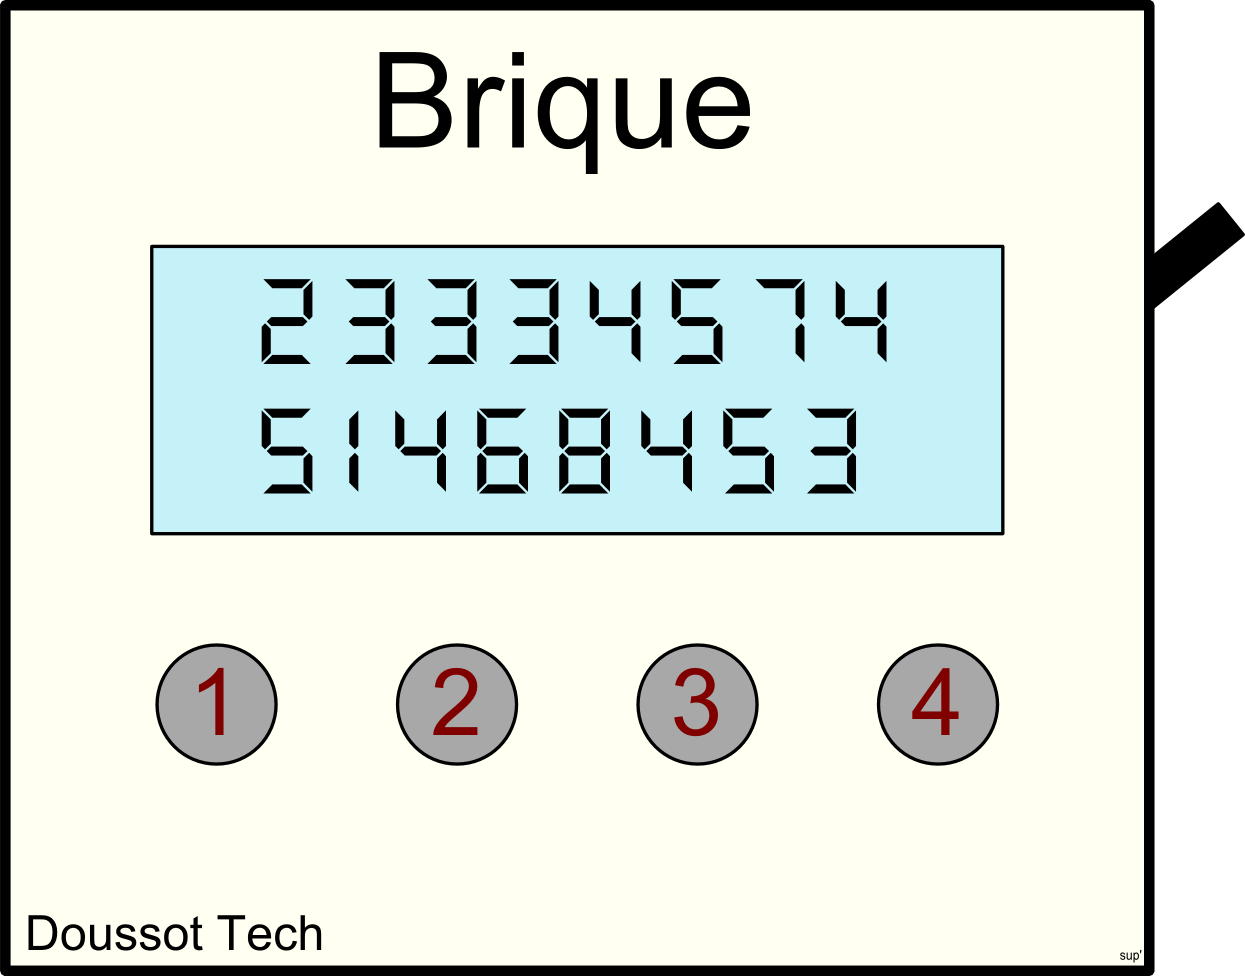
\includegraphics[width=\textwidth]{brique_dessin.png}
	\caption{Schéma de la brique}
	\label{brique_dessin}
\end{figure}

La brique se présente sous un boitier doté d'un switch sur le coté, un écran LCD et quatres boutons, qu'on nommera bouton 1, 2, 3 et 4.

\bigskip
Le switch fais passer le circuit sur un fonctionnement par pile. L'allumant à l'occasion s'il n'est pas branché.

Une première pression sur le bouton 1 lance la capture de donnée. Une deuxième pression le met en pause. Appuyer longuement sur le bouton arrête la capture.

Chaque pression sur le bouton 2 fait defiler l'affichage. Dans l'ordre, l'ecran affiche : 
\begin{itemize}
\item La distance parcourue
\item Les coordonnées
\item la vitesse
\end{itemize}

Le bouton 3 permet de changer le mode de capture.

Le bouton 4 ne permet rien. Rien ! RIEN !

\end{document}
